\section{Sensornetzwerke als Datenquellen}
Sensortechnologie wurden im Laufe des AGREE-Projekts zum wichtigsten Forschungsgebiet in der zu zukünftigen Zusammenarbeit gewählt.\cite{misc:Mikkola2013} Sensornetzwerke sind Netzwerke aus Knoten die folgende bestimmte Funktionen verfügen bzw. folgende Bestandteile haben:
\begin{itemize}
	\item Sensoren um verschiedene Umweltparameter messen zu können. (z.B. Luftdruck, Luftfeuchtigkeit, Zusammensetzung der Gase in Umgebungsluft, Helligkeit, etc.)
	\item Rechenmodule um bestimmte Kalkulationen durchzuführen um z.B. Sensorenwerte auszuwerten.
	\item Kommunikationsmodule um entweder Messungen oder (Teil-)Ergebnisse von Kalkulationen zu übermitteln. (z.B. ZigBee, Wireless Lan, etc.)
\end{itemize}
Wenn diese Funktionen um ein Modul zur Fortbewegung des Knotens erweitert wird, handelt es sich um einen mobilen Sensornetzwerkknoten.\cite{jour:Howard2002}

Die Sensormodule können je nach Einsatzzweck sowohl in kleinen, gut zu kontrollierenden Bereichen wie z.B. Glashäusern eingesetzt werden, in großflächigen Feldern oder in Ställen in der Viehhaltung. Dies ist eine notwendige Basis für sg. \textit{Context Aware Computing}-Anlagen die bestimmte Umweltparameter wie z.B. Licht, Nahrung oder Bewässerung steuern können. 

Energieeffizenz spielt für Sensorknoten im Falle von Einsätzen auf großflächigen Feldern eine besondere Rolle, da hier der Einsatz von Batterien bzw. Akkumulatoren eine Notwendigkeit ist und die Wartung bzw. das Austauschen oder Aufladen aufwendig. 

In \textit{Energy Efficient Cognitive Radio MAC Protocols for Adhoc Network: A Survey} werden drei \textit{Media Access Control}-Protokolle, kurz MAC, vorgestellt (ECR-MAC, EECR-MAC, EQR-MAC) die für den Einsatz für Adhoc-Sensornetzwerke konzipiert wurden.\cite{conf:Zia2013} In \textit{Context-Adaptive Multimodal Wireless Sensor
Network for Energy-Efficient Gas Monitoring} werden Optimierung sowohl was das Netzwerkprotokoll bis hin zum Physical Layer betrifft vorgestellt aber auch was den Energiehaushalt des Knoten selbst betrifft. Dabei wird eine Lebenszeit von mehreren Jahren für einen Knoten erreicht.\cite{jour:Jelicic2013}

In \textit{Design and Development of Precision Agriculture System Using Wireless Sensor Network} wird eine Beispiel-Implementierung eines Sensor-Netzwerks zur optimalen Wasserversorgung vorgestellt. Die Autoren kamen zu dem Ergebnis dass sowohl der Ernteertrag gsteigert werden konnte sowie Wasser-, Energie- und Arbeitsaufwand gemindert werden konnten.\cite{jour:Nandurkar2014}

Bhargava untersucht in \textit{Wireless sensor entwork based advisory system for Apple Scab prevention} nicht nur das Netzwerk am effizentesten aufgebaut werden kann, sondern geht auch auf die Auswertung der gemessenen Daten ein. Bhargava unterscheidet hier grob zwischen zwei Architekturen:
\begin{itemize}
	\item Die sg. \textit{Two-Tier-Architecture}
	\item Einem \textit{Peer to Peer Netzwerk} kurz P2P
\end{itemize}

Die Two-Tier-Architektur ist die Aufteilung von Sensor-Netzwerk und Intelligenz. Dabei sind die Tiers durch das Internet verbunden was auch die Auswertung in Cloud-Services erlauben würde. Neben dem Vorteil die Auswertung auch aus dem Betrieb auslagern zu können, erlaubt diese Aufteilung auch die Knoten langlebiger betreiben zu können. Der Autor stellt fest, dass auf den Sensorknoten eine jede Berechnung auf Kosten der verfügbaren Akkuleistung geht.\cite{jour:Bhargava2014}

\begin{figure}[h]
 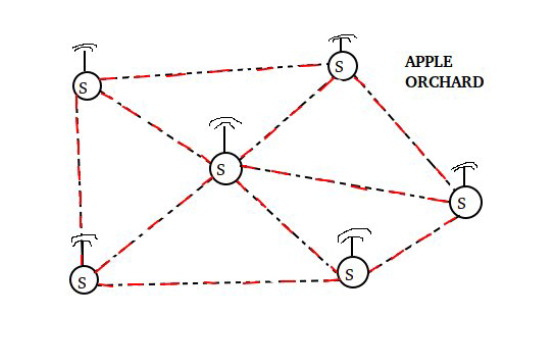
\includegraphics[scale=0.5,natwidth=\textwidth]{figures/sensors/p2p_architecture.png}
 \centering
 \label{fig:fmishierarchy}
 \caption{Vorgeschlagene Two-Tier-Architektur \cite{jour:Bhargava2014}}
\end{figure}

Im Gegensatz dazu, werden die gemessenen Daten in der P2P-Architektur im Netzwerk selbst ausgewertet. Dies hat im Vergleich zur Two-Tier-Architektur einige Nachteile:
\begin{itemize}
	\item Die Lebensdauer der verwendete Energiequelle leidet darunter und ist früher erschöpft.
	\item Es können durch die begrenzte Leistungsfähigkeit der verfügbaren Chips auf den Sensorknoten nur triviale Auswertungen durchgeführt werden.
	\item Je nach Einsatzgebiet (z.B. in gebirgigen Landschaften), kann die Verfügbarkeit der Daten nicht garantiert werden. Dies könnte bei einem Alarm dazu führen, dass dieser nur zu spät gemeldet werden kann.
\end{itemize}

\begin{figure}[h]
 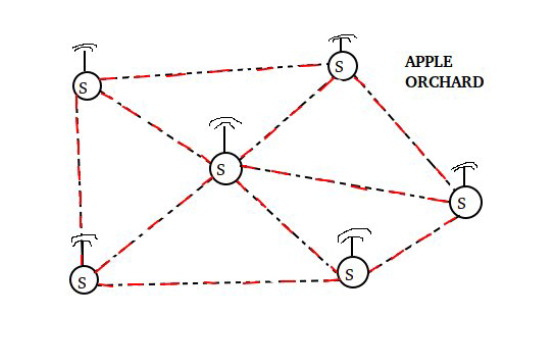
\includegraphics[scale=0.5,natwidth=\textwidth]{figures/sensors/p2p_architecture.png}
 \centering
 \label{fig:fmishierarchy}
 \caption{P2P-Struktur des Sensornetzwerks \cite{jour:Bhargava2014}}
\end{figure}

Aus diesen Gründen spricht Bhargava die Empfehlung aus, die Auswertung auf einen Server welcher über das Internet erreichbar ist auszulagern.\cite{jour:Bhargava2014}

\section{Satellitensysteme als Datenquellen}

In \textit{Estimating rice nitrogen status with satellite remote sensing in Northeast China} wird eine auf Satellitenbildern aufbauende Analyse des Reisanbaus vorgeschlagen. Dieses Vorgehen hat den Vorteil, dass zum einen die Gebiete nicht mit Sensorknoten bestückt werden müssen - was im Falle von Nassgebieten wie Reisfeldern weitere Probleme bereit hält - und dass die lokalen Messinstrumente nur über längere Zeitperioden verlässliche Daten liefern.\cite{jour:Huang2013} 

\begin{figure}[h]
 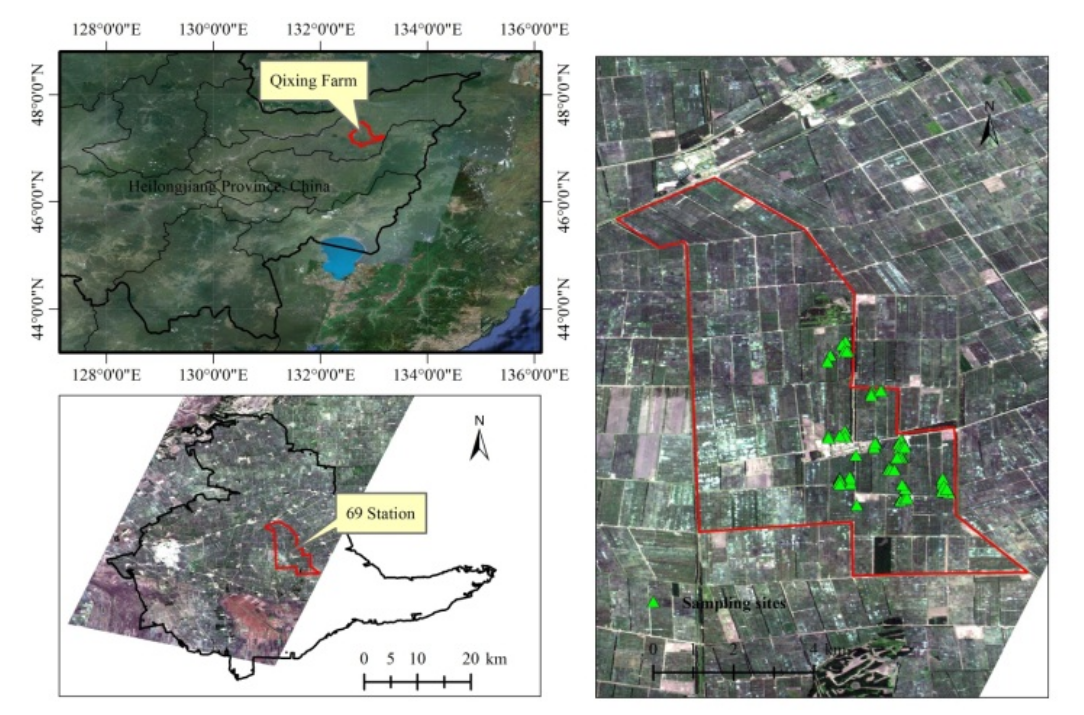
\includegraphics[scale=0.4,natwidth=\textwidth]{figures/sensors/satellite_area.png}
 \centering
 \label{fig:fmishierarchy}
 \caption{Aufnahme des Gebiets dessen Umweltwerte gemessen wurden. \cite{jour:Huang2013}}
\end{figure}
